\documentclass{article}
%\documentclass[a4paper, 11pt, left=2cm, right=2cm, top=2cm, bottom=2cm]{article}
\usepackage[left=2cm, right=2cm, top=2cm, bottom=2cm]{geometry}

\usepackage{graphicx} % Required for inserting images
\usepackage{float}

%colored text
\usepackage{xcolor}

\usepackage{biblatex}
\bibliography{sample}

\title{Deep Learning Reproducibility}
\author{Valérie van Noesel,     4874579,    V.S.vanNoesel@student.tudelft.nl \\ 
Menthe Steensma,     4941381,    M.M.Steensma@student.tudelft.nl\\ 
Matthijs Steyerberg,  4668677,   M.D.Steyerberg@student.tudelft.nl\\ 
Shantnav Agarwal,    5939933,    S.Agarwal-19@student.tudelft.nl }
\date{April $11^{th}$ 2024}

\begin{document}

\maketitle

\section{Introduction}
With the advance of modern GPUs, more complex machine learning models become feasible. In this blog, the use of generative adversarial networks (GANs) to generate faces with different poses is explored. In 2021, Eric Chan et al. \cite{chan2022efficient} published an article that provided an application of generating poses and angles of a 2D portrait image. Additionally, it creates a 3D model of the face based on the image. The code to this model is available on github \parencite{github}.\\
This paper has two main contributions. Firstly, this paper reduces model complexity by use of a hybrid representation of features on a tri-plane. Secondly, this paper decouples feature extraction and neural rendering, which makes it possible to use existing 2D models such as StyleGAN2.\\
We provide a reproducibility check by recreating outputs similar to figure 6 from the original paper. Additionally we explore the generation process to make a person's features adjustable by changing the latent vector. In this blog we will discuss the cause of background blackening and blurring at steep camera angles, by comparing two models. Also, an analysis of feature editing by changing the latent vector values and a 3D model of the eye region is generated. \\
Finally, one of the shortcomings of the proposed method is that the generated 3D model contains a concave eye model, and unrealistic eye pose in 2D: eyes keep focused on the camera, even at steep angles. The aim of our extracted 3D eye model is to facilitate further analysis and potential improvement, so that different eye poses can be generated. 

\section{Short recap of the paper}

In order to understand what the reproducibility project involves, we first start with a quick review of what has been done in the original paper. In figure \ref{fig:gan_framework}, an overview of the full 3D framework is given \cite{chan2022efficient}. The process can be split up in several steps, which will shortly be explained in this section.

\begin{figure}[H]
\centering
  \centering
  \includegraphics[width=1\linewidth]{3D GAN network.jpg}
  \caption{3D GAN framework used in the original paper \cite{chan2022efficient}}
  \label{fig:gan_framework}
\end{figure}

\begin{enumerate}
    \item \textbf{StyleGAN2-based feature generator}
    One of the advances in the paper was the decoupling of the neural rendering step from the feature generation, allowing the use of established 2D image CNNs. Here, StyleGAN2 is used, a network with a well-understood and efficient architecture that allows for style-mixing and latent-space interpolation. With the network and the camera pose parameters, features are extracted from 2D images.
    
    \item \textbf{Novel tri-plane 3D representation}
    Then, a hybrid implicit-explicit tri-plane representation such as in figure \ref{fig:triplane} is used to represent the found features. Neural implicit representations (NeRF) use fully connected layers with positional encoding, which is slow to query. Explicit voxels are fast to query, but suffer from poor scalability with regard to resolution. The combination of both, using a tri-plane, offers best of both worlds: it is fast and efficient. 

\begin{figure}[H]
    \centering
    \centering
    \includegraphics[width=0.5\linewidth]{triplane.jpg}
    \caption{Different types of feature representations \cite{chan2022efficient}}
    \label{fig:triplane}
\end{figure}

    \item \textbf{Neural volume renderer}
    A multi-layer perceptron (MLP) decoder reads out the 3D feature volume by sending out rays along which a certain amount of samples are taken. The output is a density $\sigma$ together with a 32-channel feature. With this information, 2D feature images are created.  
    
    \item \textbf{Super resolution module}
    Although the tri-plane representation allows for a speed-up, it is still too slow to train or render at higher resolutions. Therefore, a lower resolution of 128$^2$ pixels is rendered, after which the extra module is used to upsample to a higher resolution of 512$^2$ pixels.
    
    \item \textbf{StyleGAN2 discriminator with dual discrimination}
    Finally, an upgraded version of the standard StyleGAN2 discriminator is used. The camera pose from which the image is rendered is also fed to the discriminator, to make the generator effectively learn 3D priors. The dual discrimination is formed by concatenating the output image of the super resolution module with a bilinearly upsampled image. The two images together form a six-channel image instead of the regular three-channel image that is used by traditional GAN discriminators. The benefit is that multi-view inconsistency issues are resolved.
    
\end{enumerate}
\section{Steep angle analysis}
The background of the portrait images changes together with the pose. Figure \ref{fig:non_rebalanced} shows the input image in the center. All the output images are the surrounding images. When the angle becomes larger, shown in the outermost columns of figure \ref{fig:non_rebalanced}, the extremities of the background turn black. In these same images, the backside of the heads is also distorted with random colors and blurred patches. 
Using a 'rebalanced' model gives much better results, shown in figure \ref{fig:rebalanced}. For the same angles, we can see that the black background and blurring on the rear of the heads have been solved largely. \\
This effect is rather easy to explain. The original model is trained mainly on images where the person looks straight ahead into the camera, such as the middle (input) picture in figures \ref{fig:non_rebalanced} and \ref{fig:rebalanced}. This means that the model has less knowledge about side projections of human heads, what the back of the head looks like and changes in background features. \\
The rebalanced model has a more uniformly distributed training dataset \cite{github}. By comparison,  rebalanced network has more training images where the person has an angle with respect to the camera. Therefore, this model knows the features on the side and rear of the head better than the original model. Additionally, it can learn about changes in background features. This explains why the rebalanced model can extrapolate the colors of the background better, and why the backsides of the heads are no longer blurred.
\begin{figure}[H]
\centering
  \centering
  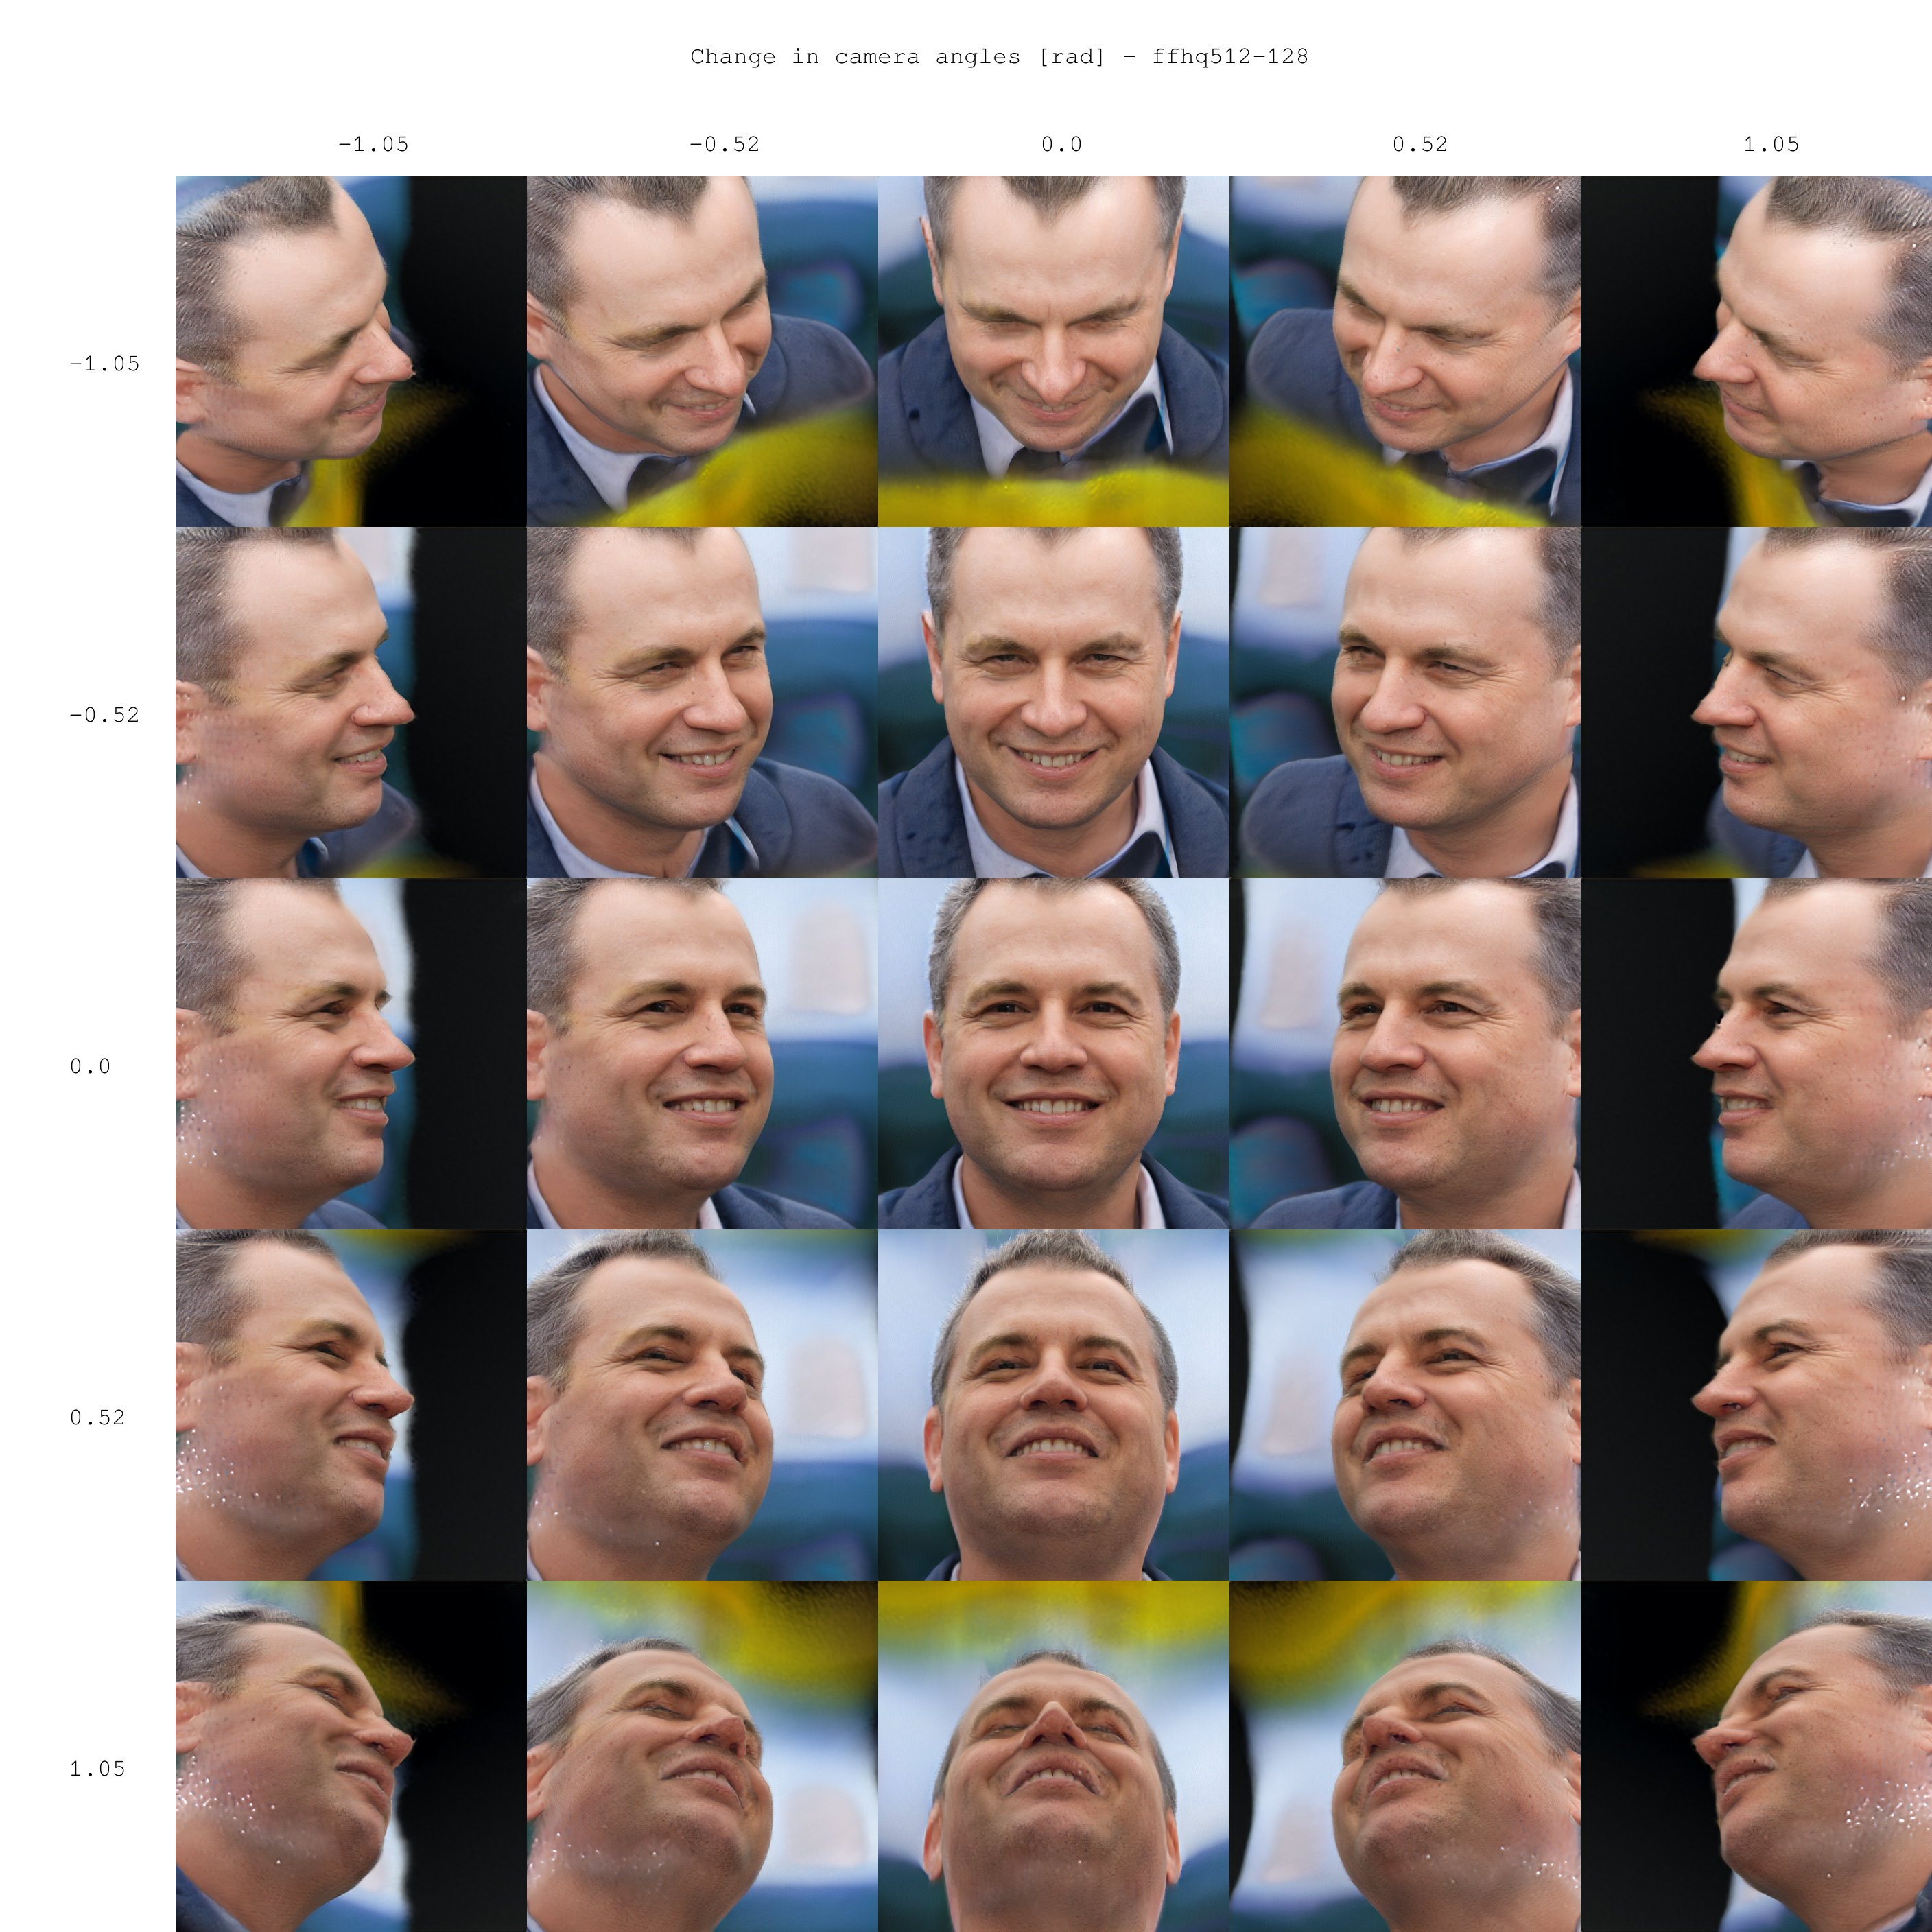
\includegraphics[width=0.6\linewidth]{angles-0001-ffhq512-128.png}
  \caption{Background with black patches using original model}
  \label{fig:non_rebalanced}
\end{figure}
\begin{figure}[H]
  \centering 
  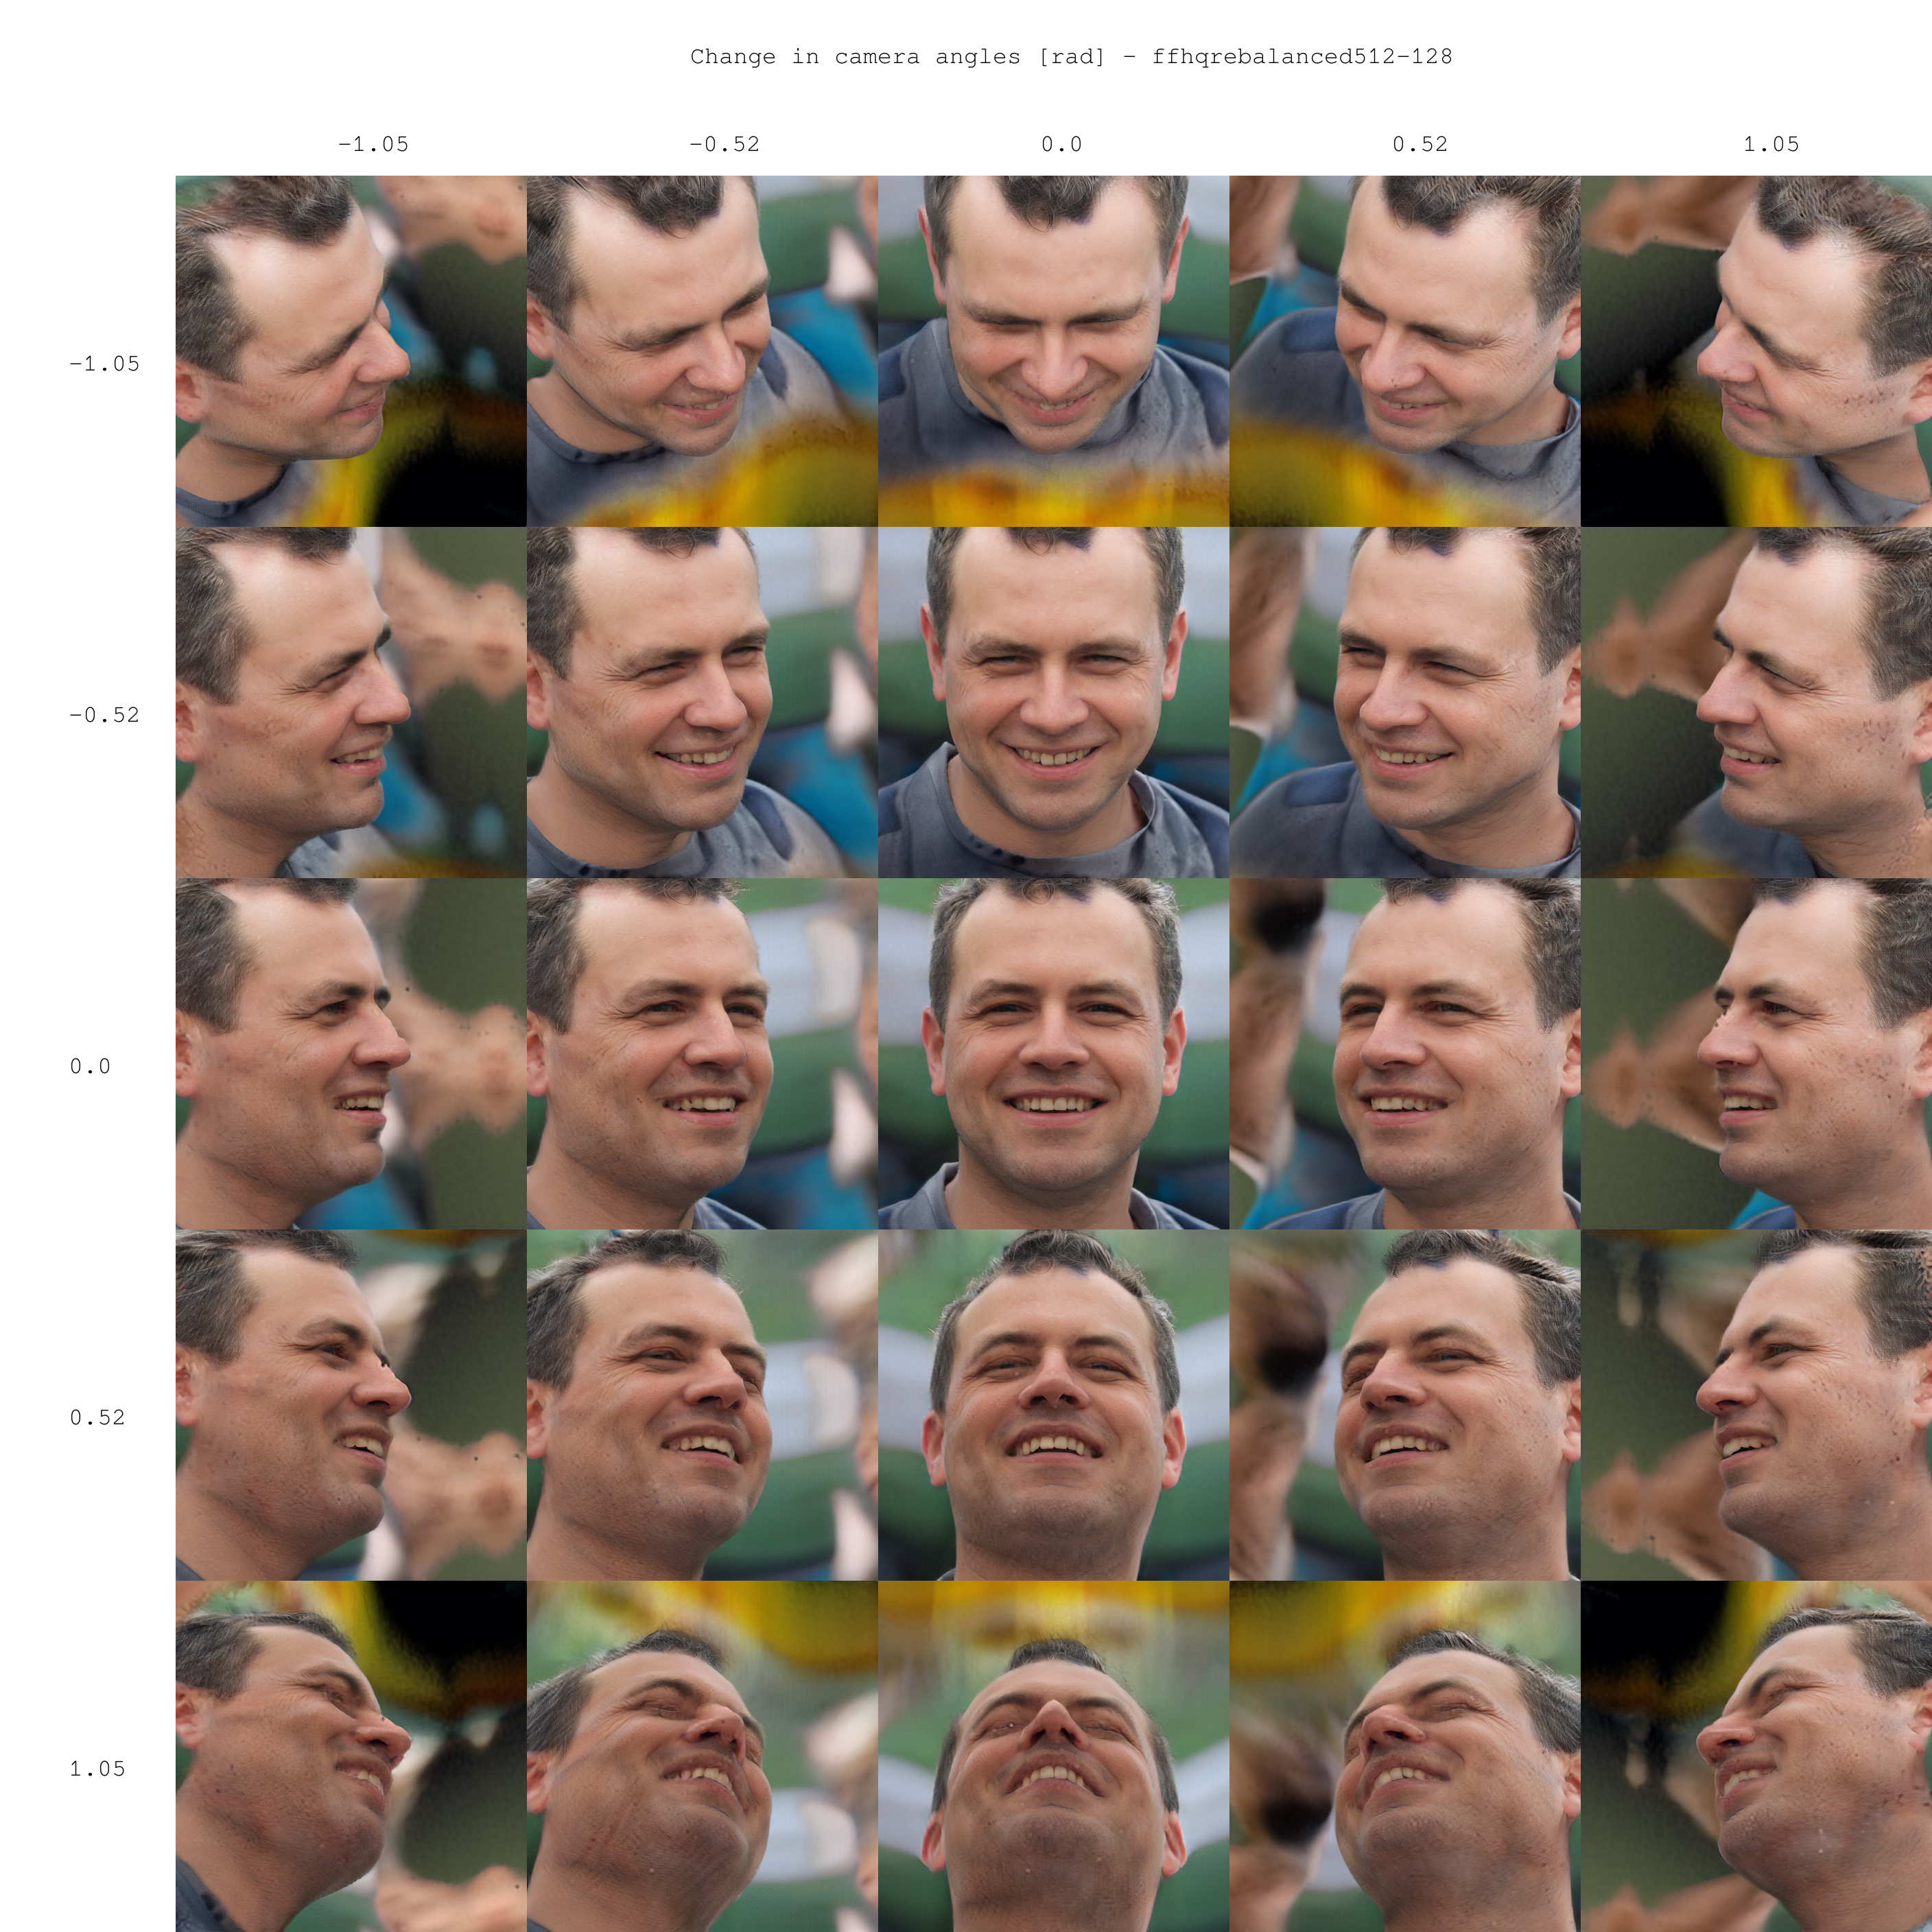
\includegraphics[width=0.6\linewidth]{angles-0001-ffhqrebalanced512-128.png}
  \caption{Background improvements using rebalanced model}
  \label{fig:rebalanced}
\end{figure}
To provide further evidence, we studied the neural volume renderer of the model to see how values of color and density cause the final rendered image to be dark where little knowledge is available. Figures \ref{fig:density_seed1} and \ref{fig:color_seed1} show the values of density and colour that are the output of the tri-plane, and are used by "volume rendering" to create the raw image. For the dark regions, we can see that the colours values are close to black, and densities are close to zero. Low volume density values particularly signify that there is no surface on which the ray will terminate. At the right side (near the back of the head) of figure \ref{fig:seed1_extreme_angle}, we see that volume density is high - correctly -, but presumably because of absence of any knowledge, the color values are unknown, and therefore close to zero (i.e. black). Together this analysis explains why the extremities of renders become black in very oblique angles.

\begin{figure}[H]
    \centering
    \includegraphics[width=0.5\linewidth]{seed0001.png}
    \caption{Rendered image with black background in the border}
    \label{fig:seed1_extreme_angle}
\end{figure}

\begin{figure}[H]
    \centering
    \includegraphics{test1blog.png}
    \caption{Variation of density values across channels. First three images are of channels equidistant from each other with the rightmost image being an average value of all channels.}
    \label{fig:density_seed1}
\end{figure}

\begin{figure}[H]
    \centering
    \includegraphics{test1cblog.png}
    \caption{Variation of color values across channels. 32 channel feature-images are output, only the first three channels are rendered}
    \label{fig:color_seed1}
\end{figure}
\section{Feature editing}

To explore the possibility of generating different facial expressions and features, we explored how different images are generated. Since the model uses StyleGAN2, it also makes use of the latent vector determining the generated image \cite{StyleGAN2}. This vector contains 512 scalar entries. To explore how each entry changes the image, we changed one entry of the latent vector at a time with five different values to explore the entire range of the scalar. The results can be seen in figure \ref{fig:changing_latent}. Although each entry of the latent vector are normally drawn from a normal distribution with standard deviation of 1, we choose to make the changes bigger in a range of [-10, 10] to show the change of the single entry more. We notice that at the extremes, the original person has completely changed into somebody else. This lead us to the exploration of the amount of truly different faces that can be generated by this model - not just the small changes such as glasses or hair length. Each latent vector entry can change the original face towards two new faces. Therefore, the amount of faces that could be generated by the model exceeds $2^{512} \approx 10^{124}$.

\begin{figure}[H]
    \centering
    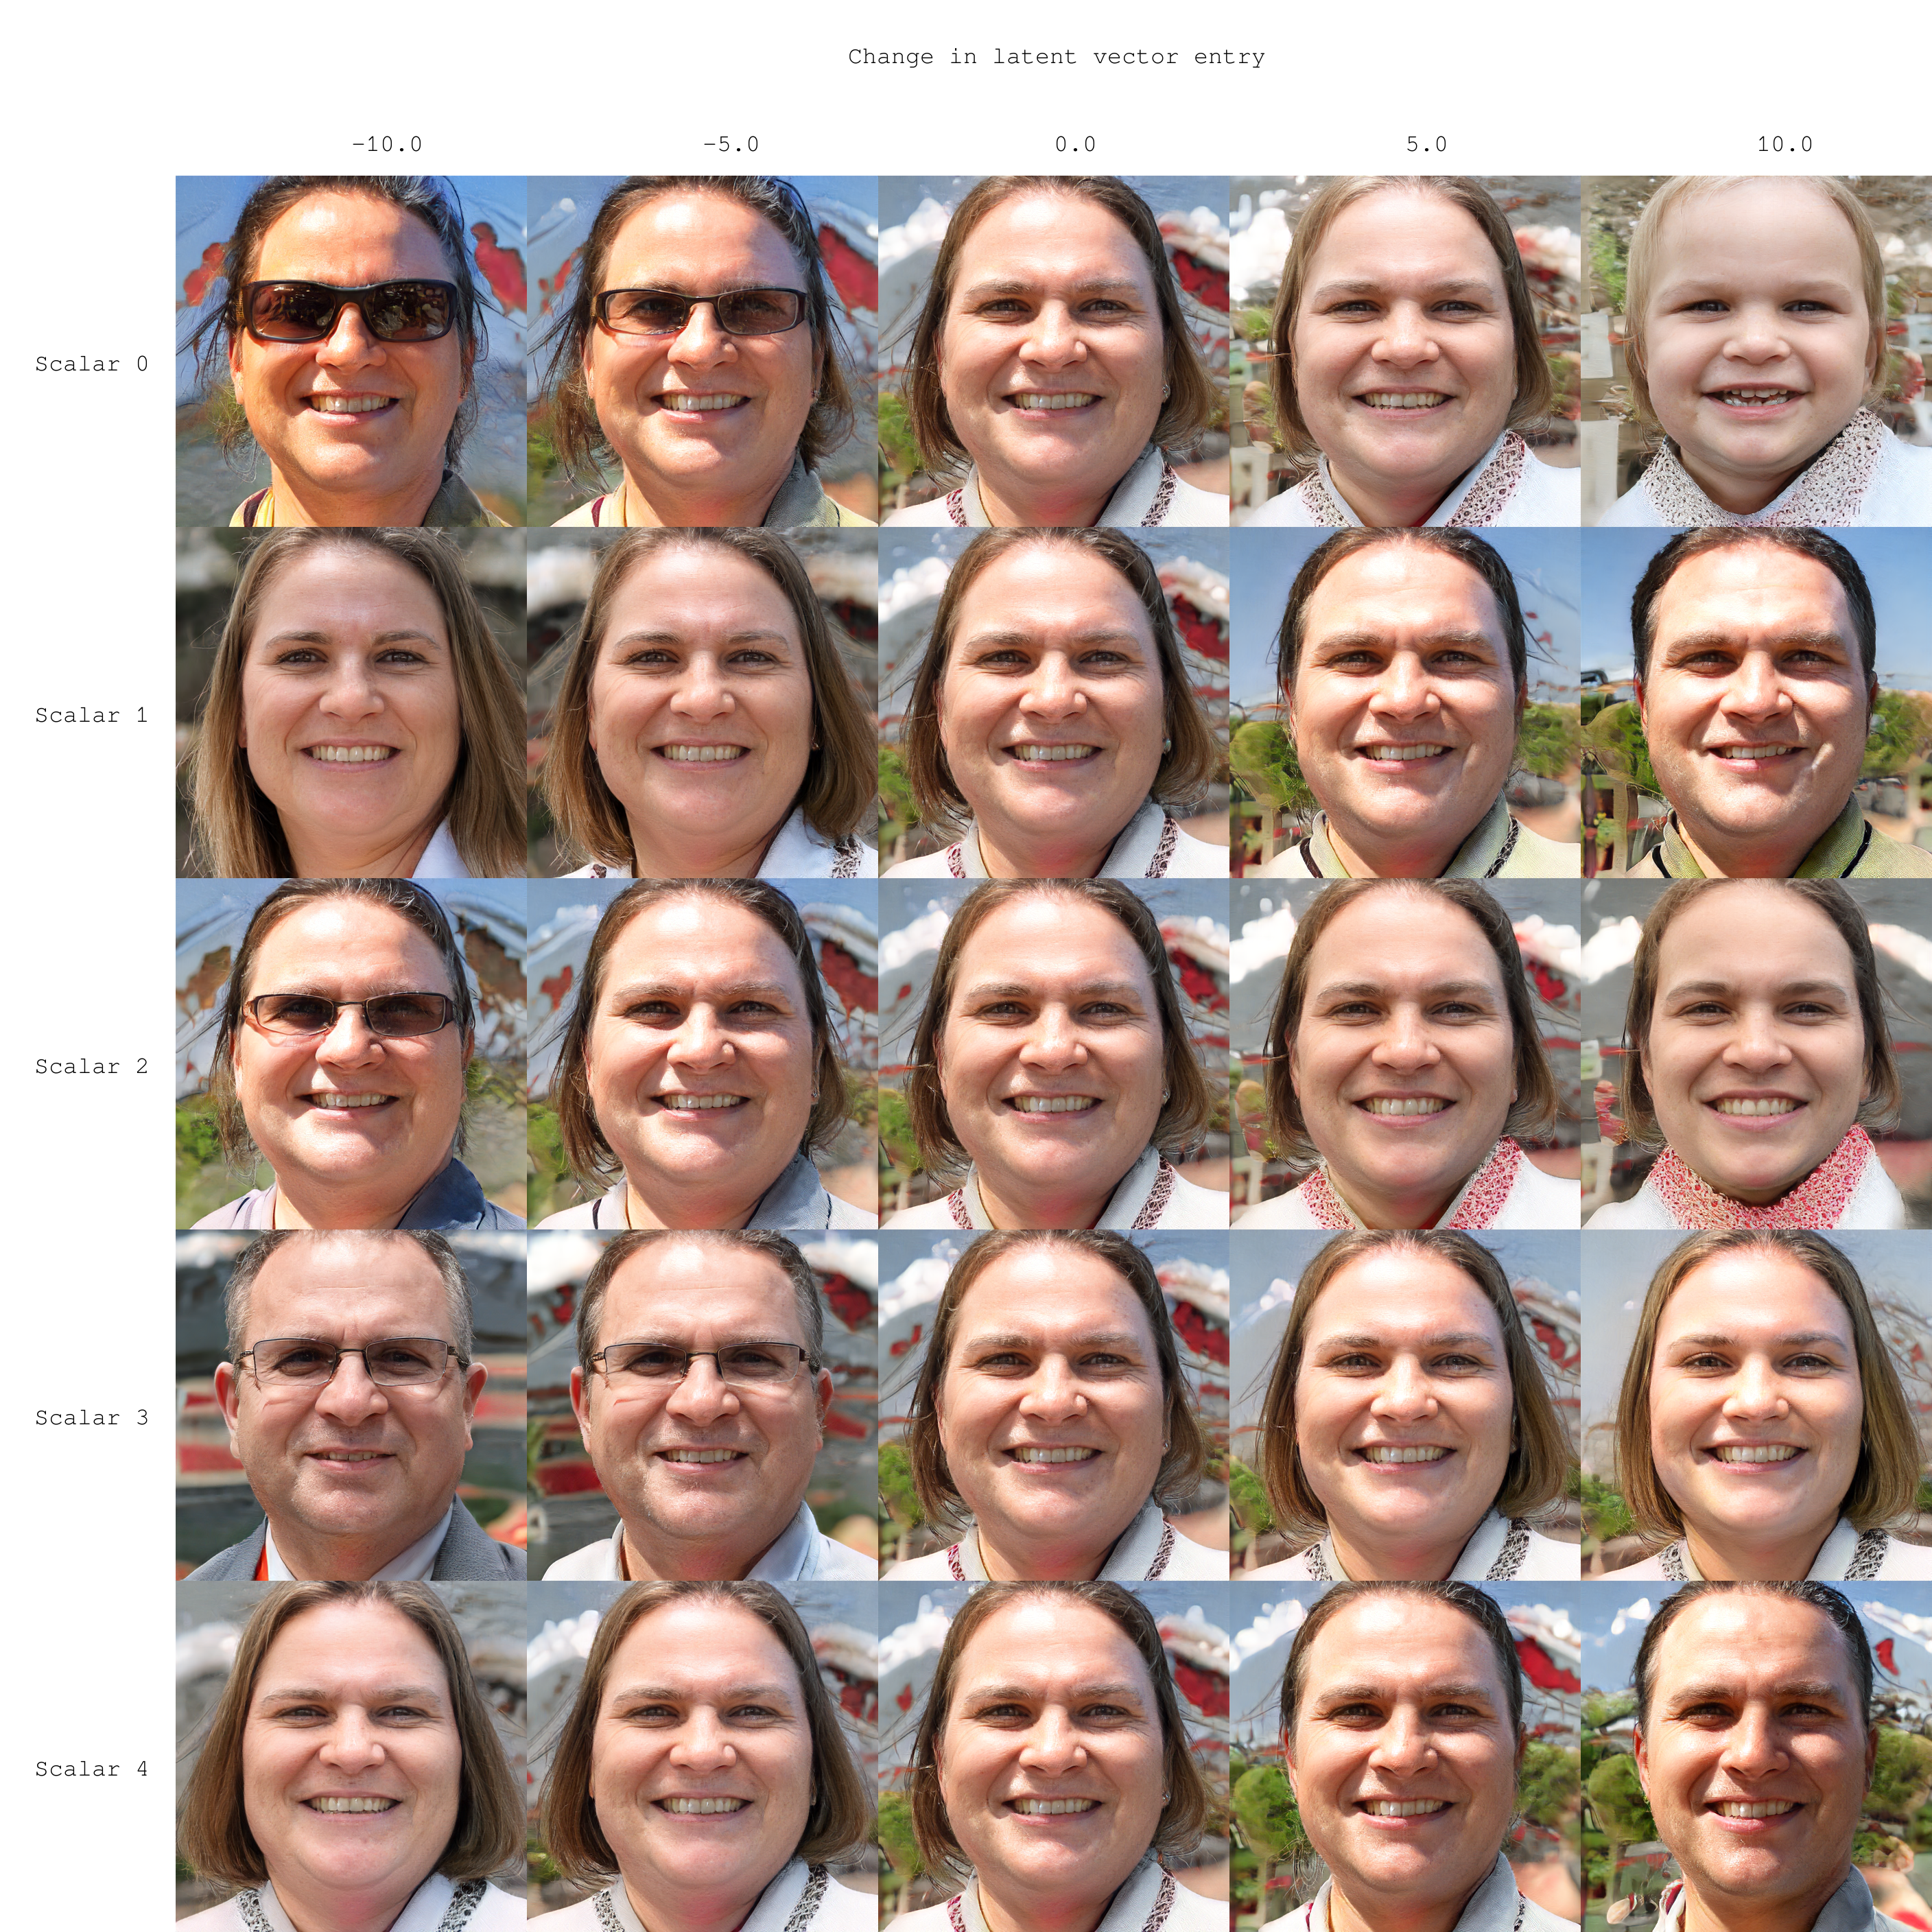
\includegraphics[width=0.9\linewidth]{latent-0004-ffhqrebalanced512-64.png}
    \caption[width=0.6]{Generated images for change in single latent vector entry. Showing the possibility to change the original image features towards different facial and background features}
    \label{fig:changing_latent}
\end{figure}
\section{Eye rendering}
One of the pitfalls of the model concerns the eye region: for different viewing angles, the eyes stay focused on the camera. In the 3D head models, it can be seen that the eye sockets are concave, shown in figure \ref{fig:concave_eyes}.

\begin{figure}[H]
\centering
  \centering
  \includegraphics[width=.9\linewidth]{concave_eyes.jpg}
  \caption{3D rendered eyes showing the concave eye area \cite{chan2022efficient}}
  \label{fig:concave_eyes}
\end{figure}

When creating the 2D images from different viewing angles, the model interprets this incorrectly, locking the eyes to the camera in every pose. A reason can not be found in literature. However, we believe the reason for this is the training data. In mostly all training images, the person looks towards the camera. Therefore the model makes all the output images look at the camera as well. This could be tested by training the model on a more uniformly distributed set of people looking towards the camera and people looking away from the camera. \\
However, a definite answer to the lower density in the eye part has not been found yet. To try to solve this problem, the first step is to prepare a dataset on this specific area. As the model is trained on the full head, it is not possible to change the model's output to only the eyes without retraining the model. Instead, the eye portion is extracted from the full 3D head and only that part is rendered with the computer graphics algorithm Marching cubes (figure \ref{fig:eye_rendering_step}). The resulting 3D model can be seen in figure \ref{fig:cropped_eyes}.

\begin{figure}[H]
\centering
  \centering
  \includegraphics[width=.6\linewidth]{eye_rendering_step.jpg}
  \caption{Framework with the additional step to extract the eye region}
  \label{fig:eye_rendering_step}
\end{figure}

\begin{figure}[H]
\centering
  \centering
  \includegraphics[width=0.7\linewidth]{Cropped eyes.jpg}
  \caption{Cropped 3D model of only the eyes}
  \label{fig:cropped_eyes}
\end{figure}

\subsection{3D Eye model}
Now that we know how to use the extracted 3D eye region, we need to find a way to obtain these 3D models. When the full head is modeled, it starts building in the bottom left corner, and adds 'blocks' in vertical strokes. To build only the eye region, we adapted the code to start at the top of the left cheek and work its way up to above the eye. By exhaustive exploration we have found that the bottom 50\% of the face is redundant. The same goes for the top 37\%. These values leave some space above and below the eyes, which is what makes them generalizable. For all faces that we have tested, the eyes fall within this region without leaving large margins on either side of the eye. For the specific changes in the code, please read the commit changes of our solution \parencite{gitcommit}.
 
\section{Small summary}
In this blog post, we delved into the possibilities enabled by modern GPUs to generate faces with various poses and characteristics based on the 2021 article by Eric Chan et al. \cite{chan2022efficient}, which showcased the creation of 3D models from 2D portrait images using GANs. We have replicated figures from the original paper, and pushed the model even further exploring more extreme angles to generate faces. Additionally, we explored the adaptability of generated features by making changes to the latent vector entries to influence the rendered person portrait. We discussed the differences between normal and rebalanced models, and identified a pitfall concerning the unrealistic concave eye rendering in generated images. To better understand this issue, we initiated a process to analyze and potentially improve the rendering of the eye region. This involves the extraction and rendering of only the eye portion of the 3D models. Overall, our exploration sheds light on both the capabilities and limitations of this GAN-based approaches in generating realistic facial images with various poses and facial features.


\section{Work distribution}

\begin{figure}[H]
    \centering
    \includegraphics[width=0.9\linewidth]{Work distribution.jpg}
    \caption[width=0.6]{Work distribution during the project}
    \label{fig:work_distribution}
\end{figure}

\printbibliography
\end{document}
